\documentclass[conference]{IEEEtran}
\IEEEoverridecommandlockouts
% The preceding line is only needed to identify funding in the first footnote. If that is unneeded, please comment it out.
\usepackage{amsmath,amssymb,amsfonts}
\usepackage{algorithmic}
\usepackage{textcomp}


\usepackage[french]{babel}
\usepackage[utf8]{inputenc}

% Add i.e and e.g commands
\usepackage{xspace} %smart handling of space in commands
\newcommand{\ie}{i.e.,\xspace{}}
\newcommand{\eg}{e.g.,\xspace{}}


\input{latexGoodPractices/preamble.tex}

\addbibresource{./bibliography.bib}

\begin{document}

\acrodef{VSS}{véhicules \textit{skid-steer}}
\acrodef{ICP}{\textit{Iterative Closest Point}}

\title{Rapport GSO-7107\\}

\author{\IEEEauthorblockN{Dominic Baril, Julien Lépine}
}

\maketitle

\begin{abstract}
Les modèles dynamiques de mouvement de véhicules sont des outils primordiaux pour le systèmes de prise de décision ainsi que pour la conduite autonome.
Pour ces modèles, les modèles de force de contact linéaires sont très souvent utilisés pour les véhicules routiers en raison de leur simplicité.
Dans ce rapport, nous montrons que ces modèles sont adéquats pour les \ac{VSS} malgré leur mouvements latéraux prononcés.
Pour valider cette hypothèse, nous comparons un modèle de force de contact linéaire avec la force centripète subie par un \ac{VSS} opérant en régime permanent.
Notre hypothèse est validée pour la conduite à une vitesse \SI{0.5}{\meter\per\second} et pour 10 vitesses angulaires distintes.
\end{abstract}

\section{Introduction}~\label{sec:intro}
Un modèle de mouvement est un outil essentiel pour plusieurs opérations qui impliquent l'utilisation d'une flotte de véhicules.
En premier lieu, un modèle de mouvement permet d'analyser les forces en jeu dans l'opération d'un véhicule et permet d'analyser l'impact de plusieurs opérations réalisées sur une flotte de véhicules.
Cette analyse d'impact permet de guider les décisions liées à une flotte de véhicules et donc d'optimiser les coûts financiers et écologiques de la flotte.
En second lieu, un modèle de mouvement est un fondement critique dans l'automatisation de la conduite de véhicules. 
Cette tâche permettrait éventuellement d'accomplir plusieurs tâches redondantes sans nécessiter la présence d'un opérateur, ce qui pourrait supporter plusieurs industries qui souffrent de la pénurie de main d'oeuvre actuelle.
% Trouver 1 ou 2 citations pour statistiques
Ces modèles peuvent prendre deux formes : cinématiques et dynamiques.
Les premiers permettent de modéliser la géométrie du mouvement des véhicules et les deuxièmes permettent de modéliser les forces agissant sur les roues des véhicules.
Les modèles dynamiques sont plus riches et permettent de modéliser une plus grande plage de conditions auxquelles les véhicules sont soumis. 

Le fondement le plus important d'un modèle de mouvement de véhicule terrestre est la géométrie de direction. 
Dans le cadre de ce cours, nous avons étudié en détails la géométrie dite \textit{Ackerman}, qui est la plus répandue pour les véhicules routiers.
Dans le cas de la conduite hors route, la géométrie \textit{skid-steer} est également très populaire.
Pour tourner ce type de véhicule, une différence de vitesse de rotation entre les roues de chaque côté du véhicule est imposée. 
Les \ac{VSS} offrent plusieurs avantages, notamment la simplicité mécanique, la robustesse, la manoeuvrabilité hors route et la capacité de tourner sur place~\citep{Shamah2001}.
Toutefois, ces véhicules sont soumis à une friction latérale élevée puisque les roues sont constamment parallèles à la direction longitudinale du véhicule. 
Comme les modèles de force de contact linéaires sont populaires pour les véhicules \textit{Ackerman}, il serait pertinent d'évaluer leur performance pour les \ac{VSS}, comme ceux-ci sont soumis à des forces latérales élevées.

Les contributions liées à ce rapport sont donc :
\begin{itemize}
	\item La formulation d'un modèle dynamique planaire de \ac{VSS};
	\item L'évaluation de l'exactitude d'un modèle de force de contact linéaire pour les forces latérales subies par le robot.
\end{itemize}
La structure du rapport est comme suit :
Une revue de la littérature connexe à ce travail est présentée dans la~\autoref{sec:revue}.
La~\autoref{sec:metho} explique la méthodologie utilisée pour atteindre les contributions de ce travail.
Les résultats sont présentés dans la~\autoref{sec:resultats}.
Une analyse détaillée des résultats suit à la~\autoref{sec:analyse}.
Enfin, une conclusion et les travaux futurs sont présentés dans la~\autoref{sec:conclu}.
\section{Revue de littérature}~\label{sec:revue}
Afin de montrer la pertinence de ce travail dans la littérature, nous montront les techniques de modélisation du mouvement pour les \ac{VSS} les plus populaires dans la littérature dans la~\autoref{sec:revue_planaires}. 
Ensuite, nous présentons les travaux pertinents par rapport aux forces de contact dans la~\autoref{sec:revue_contact}.

\subsection{Modèles de mouvement}~\label{sec:revue_planaires}
La modélisation du mouvement des \ac{VSS} est un problème actuel dans la littérature scientifique.
En raison de leur simplicité et de leur résilience à l'identification de paramètres éronnée, les modèles cinématiques empiriques sont actuellement les plus populaires, tel que celui présenté par~\citet{Mandow2007}.
Alternativement, le modèle présenté par~\citet{Seegmiller2014} permet de modéliser le comportement dynamique du robot comme des perturbations subies par un modèle cinématique simple connaît également de la popularité dans la littérature.

Bien que simples, ces modèles font l'hypothèse que le robot navigue sur un terrain plat et dur, ce qui est généralement faux dans le cadre de la conduite hors route.
\citet{Rabiee2019} ont introduit un modèle croisé entre la cinématique et la dynamique.
Dans ce modèle, l'accélération des roues sont utilisées pour minimiser le système d'équations de la dynamique du corps du \ac{VSS}.
Une fois le système d'équations minimisé, les valeurs sont introduites dans un modèle cinématique analogique à~\citep{Mandow2007} pour prédire le déplacement du véhicule.
Alternativement, \citet{Seegmiller2016} ont présenté une formulation générale permettant de modéliser le mouvement de tout types de véhicules en minimisant le calcul et en offrant une grande précision.

\subsection{Forces de contact}~\label{sec:revue_contact}
Tous les modèles dynamiques de véhicules nécessitent de modéliser les forces de contact des roues des véhicules.
Il existe un grand nombre de ce genre de modèles dans la littérature ainsi qu'une grande variété dans leur complexité.
Le modèle le plus simple est le modèle linéaire, qui assume une relation linéaire entre la vitesse du point de contact et la force de friction des roues~\citep{Pacejka2012}. 
Un second modèle populaire est appelé la \textit{Magic Formula}, proposé par~\citet{Pacejka2012}.
Ce modèle empirique permet de modéliser la perte de friction causée par le passage de friction statique à friction dynamique et est très populaire pour les véhicules routiers~\citep{Brach2011}.
Une adaptation pour un \ac{VSS} a également été proposée par~\citet{Maclaurin2011}.
Dans ce travail, l'auteur évalue les paramètres du modèle empirique en fonction de propriétés physiques d'un \ac{VSS} lourd.

Des modèles plus complexes basés sur l'interaction entre les roues et le sol ont aussi été proposés.
La majorité de ces modèles sont basés sur des travaux pionniers de~\citet{Wong1967}.
\citet{Ishigami2007} ont proposé un modèle de force de contact permettant de modéliser les forces latérales. 

Bien que plusieurs modèles complexes ont été proposés pour modéliser les forces de contact, les résultats montrés par~\citet{Seegmiller2016} suggèrent que les modèles linéaires offrent une erreur de modélisation inférieure aux autres modèles sur une longue trajectoire.
Notre hypothèse est que le nombre élevé de paramètres utilisés dans ces modèles affecte la capacité aux modèles de généraliser sur un grand nombre de conditions différentes.
Dans ce rapport, nous visons à évaluer l'exactitude des modèles de force de contact linéaires pour modéliser le mouvement des \acp{VSS}.

\section{Méthodologie}~\label{sec:metho}
Afin de permettre valider l'hypothèse que les modèles de force de contact linéaires sont adéquats pour les~\ac{VSS}, un modèle dynamique planaire est détaillé dans la~\autoref{sec:modele}.
Un protocole expérimental permettant d'obtenir les données nécessaires à l'évaluation des forces a été mis en place et exécuté.
Ce protocole est présenté dans la~\autoref{sec:protocole}.

\subsection{Théorie}~\label{sec:modele}
Afin d'évaluer l'exactitude des modèles de forces de contact linéaires, nous avons développé un modèle dynamique planaire de \ac{VSS}, qui est montré dans la~\autoref{fig:modele}.
Un repère global ainsi qu'un repère du corps du robot sont définis.
La totalité des quantités définies dans cette section sont exprimées dans le repère du corps du robot.
La vitesse de rotation des roues de gauche $\omega_l$ sont identiques, il en est de même pour la vitesse de rotation des roues de droite $\omega_r$. 
Il est important de noter que bien que le modèle illustré sur la~\autoref{fig:modele} ne comporte que deux roues, ce modèle fonctionne pour tout \ac{VSS} comportant deux roues ou plus sur chaque côté.
La vitesse du corps du véhicule $\bm v = [v_x, v_y]^T$ comporte une composante longitudinale et une composante latérale.
Le corps du robot a également une vitesse angulaire $\omega$.

\begin{figure}[htpb]
	\centering
	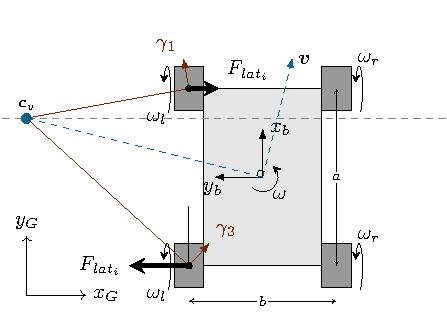
\includegraphics[width=0.48\textwidth]{figs/modele.pdf}
	\caption{Modèle dynamique planaire d'un \ac{VSS}.
			Le vecteur de vitesse du corps du robot ainsi que le centre de rotation instantané sont illustrés en bleu.
			Les angles de glissement sont illustrés en rouge.
			Dans ce modèle, seules les forces latérales subies par les roues sont considérées.}
	\label{fig:modele}
\end{figure}

En fonction de la vitesse du corps du robot, il est possible de définir la position d'un centre de rotation instantané $\bm c_v$.
La position de ce centre de centre de rotation instantané est calculée comme dans~\citep{Mandow2007} :
\begin{equation}
	\bm c_v = \begin{bmatrix}
	x_{c_v} \\ 
	y_{c_v} \\
	\end{bmatrix} = \begin{bmatrix}
	\frac{v_y}{\omega} \\ 
	\frac{v_x}{\omega} \\
	\end{bmatrix} \text{,}
	\label{eqn:icr}
\end{equation}
où $x_{c_v}$ et $y_{c_v}$ sont les positions longitudinale et latérale du centre de rotation instantané dans le repère du corps du véhicule.

Afin de simplifier le modèle, seules les forces latérales subies par le véhicule sont prises en compte.
Ces forces ont une orientation contraire à l'angle de dérive de chaque roue $\gamma_i$, qui peut être calculé ainsi, comme dans~\citep{Maclaurin2011} :
\begin{equation}
\begin{cases}
	\gamma_i = \arctan(\frac{a_i - x_{c_v}}{y_{c_v} - b_i}), & \text{if } b_i y_{c_v} > 0 \text{ et } b_i > y_{c_v} \\
	\gamma_i = \arctan(\frac{a_i - x_{c_v}}{b_i - y_{c_v}}) & \text{autrement} \text{,}
\end{cases}
\label{eqn:angles}
\end{equation}
où $a_i$ et $b_i$ sont les positions longitudinales et latérales du point de contact de la roue $i$ dans le repère du véhicule.

Ces positions sont positives ou négatives dépendant de la roue en question.
La condition est introduite afin de prendre en compte le cas où le centre de rotation instantané est situé entre les roues du véhicules.
Dans ce cas, l'angle de dérive des roues internes doit être calculé autrement.
Les forces de contact latérales subies par chaque roue $F_{lat_i}$ peuvent ensuite être calculé selon le modèle linéaire :
\begin{equation}
	F_{lat_i} = -\alpha_{lat} \gamma_i \text{,}
	\label{eqn:forces}
\end{equation}
où $\alpha_{lat}$ est un coefficient de friction lié à la nature du sol sur lequel le robot opère.
Comme les forces latérales sont des forces de friction, celles-ci sont de sens opposé à la direction du mouvement donc à l'angle de dérive. 
Alternativement, les forces latérales peuvent être calculé en substituant l'angle de dérive par la vitesse latérale du point de contact $v_{c_i}$ de chaque roue dans l'\autoref{eqn:forces}~\citep{Seegmiller2016}.
De cette manière, il est possible d'exprimer le système d'équations du mouvement dans la direction latérale du robot :
\begin{equation}
	\sum_{i=1}^{n} F_{lat_i} = m a_{lat} \text{,}
	\label{eqn:forces_sum}
\end{equation}
où $m$ est la masse du véhicule, $a_{lat}$ est son accélération latérale et $n$ est son nombre de roues total.

Pour ce modèle, nous considérons que le véhicule opère en régime permanent, ce qui implique que les accélérations longitudinale et angulaire sont nulles.
Pour ce qui est de l'accélération latérale, celle-ci est équivalent à l'accélération centripète ou d'Alembert, que l'on calcule comme~\citep{Maclaurin2011} :
\begin{equation}
	a_{lat} = m \frac{v^2}{R_c} = \frac{v^2}{\sqrt{x_{c_v}^2 + y_{c_v}^2}} \text{,}
	\label{eqn:centripete}
\end{equation}
où $R_c$ est le rayon de courbure du véhicule. 

Dans le cas où le modèle de force de contact linéaire présenté dans l'\autoref{eqn:forces} est exact, l'égalité présentée à l'\autoref{eqn:forces_sum} doit être respectée.
Il est certain qu'en raison des incertitudes liées à l'opération d'un véhicule et au bruit de capteurs, celle-ci ne sera pas respectée mais ce rapport vise à quantifier l'erreur liée à ce genre de modèle pour les \ac{VSS}.

\subsection{Protocole expérimental}~\label{sec:protocole}
Afin d'évaluer l'égalité l'exactitude du modèle présenté dans la~\autoref{sec:modele}, nous avons enregistré des données de conduite avec un \ac{VSS}. 
Un Warthog de la compagnie \textit{Clearpath Robotics} a été utilisé, une photo de cette plateforme est montrée sur la figure~\autoref{fig:warthog}.
Cette plateforme est un \ac{VSS} à 4 roues et ayant une masse $m$ de \SI{260}{\kg}.
Afin de valider notre hypothèse pour plusieurs vitesses angulaires, nous avons défini 10 vitesses angulaires commandées distintes pour l'expérience.
Ces vitesses commandées sont définies dans le vecteur $\omega_c = [0.0, 0.1, 0.2, 0.4, 0.75 ,1.25, 2.0, 3.0, 4.0, 5.0]$.
La sélection de ces vitesses a été faite dans le but d'évaluer une plus grande quantité de vitesses angulaires faibles et tenter d'observer le point de saturation des pneus.
Afin d'éviter les phénomènes liés à la déformation du terrain pour les vitesses angulaires élevées, nous avons classé les éléments de $\omega_c$ de manière aléatoire.
Pour ce qui est de la vitesse longitudinale commandée, celle-ci a été fixée à \SI{0.5}{\m\per\second} afin de limiter la longueur de l'expérience.
Pour respecter l'hypothèse de régime permanent, chaque commande a été exécutée par le robot pour une durée de \SI{10}{\second}.

\begin{figure}[htpb]
	\centering
	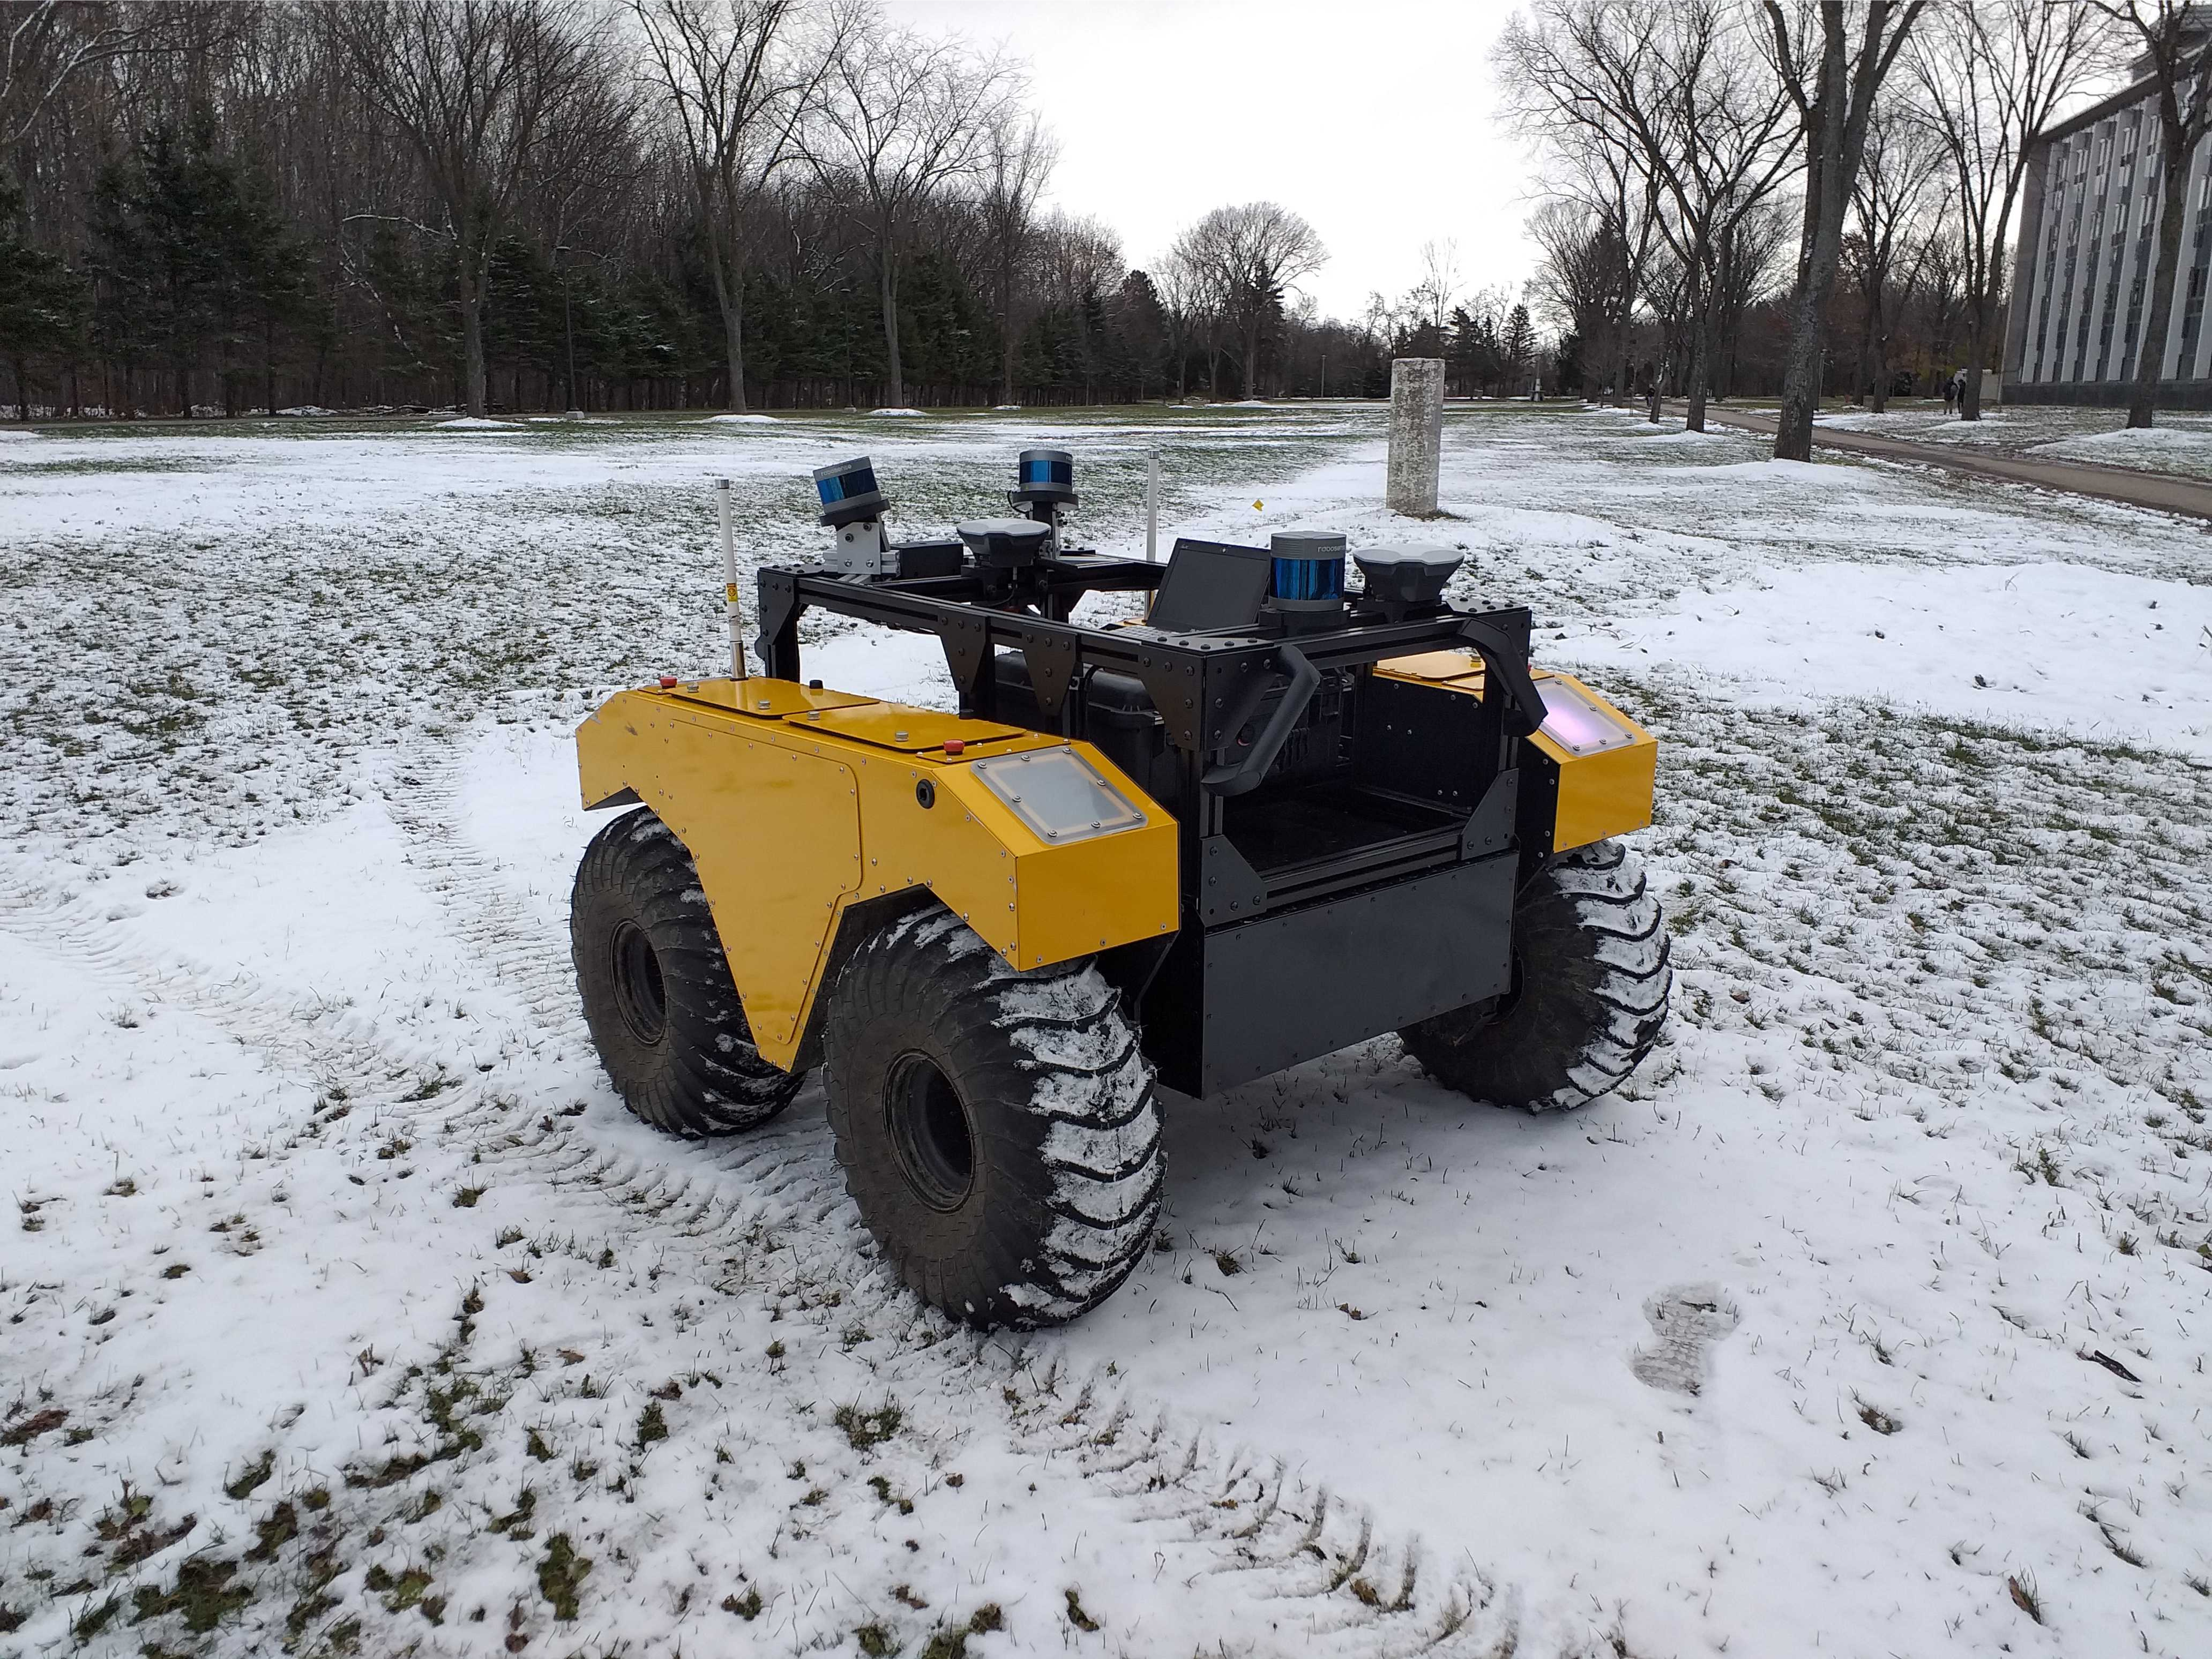
\includegraphics[width=0.4\textwidth]{figs/warthog.pdf}
	\caption{Photo du Warthog utilisé pour la phase expérimentale de ce projet.
		Cette plateforme est équipée d'un lidar Robosense RS-32 et d'une centrale inertielle Xsens MTi-10 pour se localiser.
		Le véhicule a été conduit sur le grand axe du campus de l'Université Laval, à Québec au mois de Novembre.}
	\label{fig:warthog}
\end{figure}

La plateforme comporte des encodeurs aux roues qui permettent de mesurer leur vitesse angulaire.
Une centrale inertielle permet quand à elle de mesurer la vitesse angulaire du corps du véhicule.
L'estimation de la position du corps du véhicule est réalisée en recallant des nuages de points grâce à l'algorithme \ac{ICP}~\citep{Pomerleau2015}.
La librairie \texttt{libpointmatcher}\footnote{\url{https://github.com/ethz-asl/libpointmatcher}} a été utilisée pour implémenter cet algorithme dans le cadre ce cette expérience.
Toutes les données sont enregistrées et exportées grâce au logiciel de gestion de flux de données Robot Operating System (ROS)\footnote{\url{https://www.ros.org/}}.
Le traitement des données a été réalisé grâce au langage de programmation \texttt{Python} et le code est disponible en ligne\footnote{\url{https://github.com/DomBaril/GSO-7107}}.
\section{Résultats}~\label{sec:resultats}
Un pré-traitement des données est présenté dans la~\autoref{sec:pre-traitement} afin d'évaluer la vitesse du corps du robot en filtrant le bruit.
Ensuite, les données sont utilisées pour évaluer le modèle présenté dans la~\autoref{sec:forces}.

\subsection{Pré-traitement des données}~\label{sec:pre-traitement}
En premier lieu, un traitement des données a été effectué afin d'extraire les vitesses des roues ainsi que du corps du véhicule.
Afin de respecter l'hypothèse de régime permanent et pour filtrer le bruit dans la récolte de données, la médiane de chaque valeur a été conservée pour chaque fenêtre de \SI{10}{\second}.
Suite à ce pré-traitement, le vecteur de viteses du corps du véhicule $\bm v$ et sa vitesse angulaire $\omega$ sont évalués pour chaque vitesse angulaire commandée $\omega_c$, les résultats sont montrés dans la~\autoref{fig:vitesses}.
Le vecteur $\bm v$ est mesuré à l'aide de l'algorithme \ac{ICP} et les vitesses angulaires $\omega$ sont mesurées avec la centrale inertielle.
Un modèle différentiel idéal a été utilisé pour calculer les vitesses du corps du robot en fonction des vitesses de roues. 
Ce modèle ne permet pas de modéliser la vitesse latérale du robot, ce qui explique pourquoi cette valeur demeure nulle.

\begin{figure}[htpb]
	\centering
	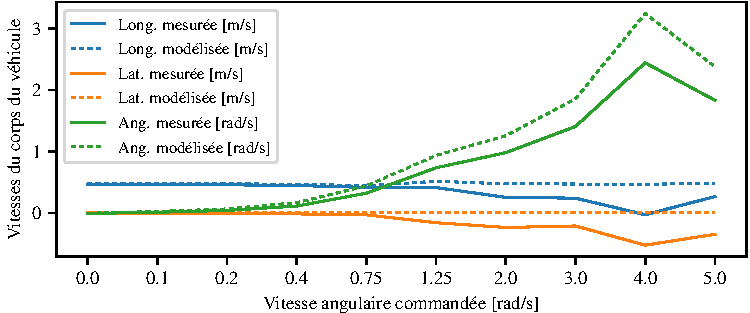
\includegraphics[width=0.48\textwidth]{figs/body_vels.pdf}
	\caption{Vitesses du corps du véhicule mesurées et modélisées dans le cadre de l'expérience en fonction de la vitesse angulaire commandée.
			La vitesse longitudinale est affichée en bleu, la vitesse latérale en orange et la vitesse angulaire en vert.
			Les vitesses mesurées avec \ac{ICP} sont montrées en lignes pleines. 
			Les vitesses estimées en fonction des vitesses des roues et d'un modèle différentiel idéal sont montrées en pointillé.}
	\label{fig:vitesses}
\end{figure}

\subsection{Évaluation des forces}~\label{sec:forces}
En premier, il est nécessaire d'évaluer les données qui vont en entrée du modèle de force de contact. 
En fonction des vitesses du corps du robot, la position du centre de rotation instantané est calculée en suivant l'\autoref{eqn:icr}.
Ensuite, les angles de dérive de chaque roue sont évalués, ceux-ci sont montrés dans la~\autoref{fig:angles}.
Dans cette figure, les angles de dérive $\gamma_i$ sont mesurés avec \ac{ICP} et modélisés en fonction des vitesses de roues et du modèle différentiel idéal.
Il est possible d'observer qu'en fonction de l'augmentation de vitesse angulaire commandée, l'angle de dérive augmente, jusqu'à plafonner et se stabiliser. 
Le pic d'angle de dérive pour les roues 1 et 3 semble se produire légèrement après le passage du centre de rotation instantané à l'intérieur de l'empattement du \ac{VSS}.

\begin{figure}[htpb]
	\centering
	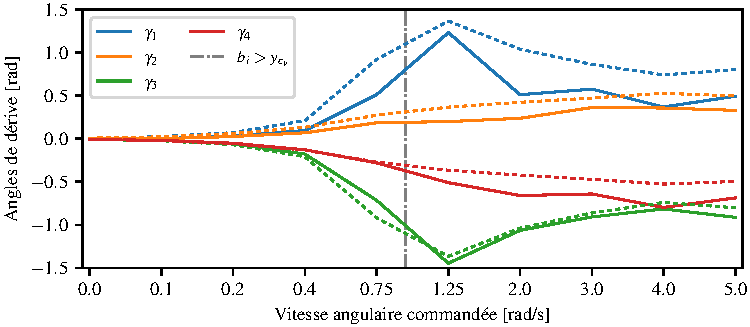
\includegraphics[width=0.48\textwidth]{figs/slip_angles.pdf}
	\caption{Angles de dérives pour chaque roue en fonction de la vitesse angulaire commandée pendant l'expérience.
			La roue 1 (en bleu) est à l'avant-gauche, la roue 2 (en orange) est à l'avant-droite, la roue 3 (en vert) est à l'arrière-gauche et la roue 4 (en rouge) est à l'arrière-droite.
			Encore une fois, les valeurs mesurées avec \ac{ICP} sont montrées avec des lignes pleines et les valeurs modélisées avec les vitesses de roues en pointillés.
			La ligne grise représente le moment où le centre de rotation instantané $\bm c_v$ se trouve entre les roues du véhicule.}
	\label{fig:angles}
\end{figure}

Ensuite, ces angles de dérive sont utilisés avec le modèle linéaire présenté dans l'\autoref{eqn:forces}.
La somme des forces latérales subies par le robot ainsi que son accélération centripète peuvent donc être calculées et l'égalité de l'\autoref{eqn:forces_sum} peut être vérifiée.
Les résultats pour les deux côtés de l'équation sont présentés dans la~\autoref{fig:acceleration}.
Afin de pouvoir calculer le modèle linéaire, une calibration manuelle a été faite pour déterminer la valeur du coefficient linéaire $\alpha_{lat}$ qui minimise l'erreur du modèle.
Ces valeurs sont similaires pour les angles de dérive (\ie~$\alpha_{lat} = 32$) ou les vitesses latérales (\ie~$\alpha_{lat} = 30$).

La force centripète est affichée en bleu et la somme des forces latérales subies par le véhicule est montrée en orange.
Comme mentionné dans la~\autoref{sec:modele}, nous avons observé que plusieurs articles dans l'état de l'art calculent les forces de contact en remplaçant l'angle de dérive par la vitesse latérale du point de contact de la roue.
La somme des forces calculées avec les vitesses latérales est affichée en vert.
Les forces ont été calculées avec les mesures d'\ac{ICP} ainsi qu'en utilisant les vitesses de roues.
Comme le modèle différentiel ne permet pas de vitesses latérales, la somme des forces latérales calculées avec les vitesses de roues est toujours nulle.

\begin{figure}[htpb]
	\centering
	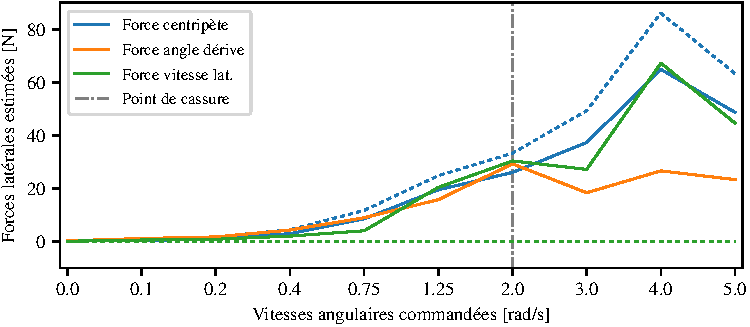
\includegraphics[width=0.48\textwidth]{figs/lateral_forces.pdf}
	\caption{Forces subies par le corps du véhicule en fonction des vitesses angulaire commandées pendant l'expérience.
			La force centripète est affichée en bleu, la somme des forces latérales calculées avec l'angle de dérive est montrée en orange et la somme des forces latérales calculées avec la vitesse latérale du point de contact est affichée en vert.
			Comme pour les figures précédentes, les valeurs mesurées avec \ac{ICP} sont montrées en lignes pleines et les forces calculées en fonction des vitesses de roues et le modèle différentiel idéal en pointillé.
			Pour les forces calculées avec un angle de dérive, il est possible d'observer un point de cassure montré avec la ligne verticale grise.}
	\label{fig:acceleration}
\end{figure}

Il est possible d'observer une faible disparité entre la force centripète et les forces calculées avec un modèle linéaire dans la~\author{fig:acceleration}.
De plus, il est possible d'observer un point de cassure à une vitesse angulaire commandée de \SI{2.0}{\radian\per\second}.
À cette vitesse, il est possible d'observer un pic dans la force centripète, qui peut être modélisé avec les vitesses de contact latérales, mais pas avec l'angle de dérive.

\section{Analyse}~\label{sec:analyse}
Dans cette section, nous analysons et discutons des résultats présentés dans la~\autoref{sec:resultats}.
Eu premier lieu, nous exposons les limites des modèles linéaires et proposons des améliorations au protocole expérimental de ce projet dans la~\autoref{sec:ana_limites}.
Deuxièmement, nous rappellons les avantages d'utiliser un modèle simple et argumentons que ceux-ci sont adéquats pour modéliser les forces subies pas les roues d'un \ac{VSS} dans la~\autoref{sec:ana_lineaire}.

\subsection{Viabilité et limites des modèles et du protocole expérimental}~\label{sec:ana_limites}
En observant la~\autoref{fig:acceleration}, on comprend que les modèles de force de contact linéaires permettent de modéliser l'accélération centripète mesurée par l'algorithme \ac{ICP}.
En effet, pour une vitesse angulaire commandée inférieure à \SI{2.0}{\radian\per\second}, les modèles linéaires basés sur l'angle de dérive ou la vitesse du point de contact sont adéquats.
Pour une vitesse angulaire commandée supérieure à \SI{2.0}{\radian\per\second}, la force estimée par l'angle de dérive semble stagner. 
Notre hypothèse pour expliquer ce phénomène est que le bruit de localization du véhicule entraîne une incertitude dans le calcul du centre de rotation instantané $\bm c_v$.
Cette incertitude est transmise dans le calcul des angles de dérive, qui sont affichés à la~\autoref{fig:angles}.
Une seconde explication pour ce phénomène est l'hypothèse que le point de cassure correspond au point de saturation du pneu du \ac{VSS} quand il opère sur le terrain identifié pour l'expérience.
Une fois passé, le véhicule se trouve en dérappage, ce qui est connu comme un phénomène complexe à modéliser.

Nous observons donc une limite fonctionnelle des modèles de force de contact linéaires basés sur l'angle de dérive à une vitesse angulaire commandée de \SI{2.0}{\radian\per\second}.
Dans l'optique où nous désirons opérer le \ac{VSS} à une vitesse angulaire supérieure, un modèle plus complexe devrait être étudié.
Il est quand même important de noter que pour la grande majorité de leur temps d'opération, les \ac{VSS} ne tournent pas à une vitesse angulaire supérieure à \SI{2.0}{\radian\per\second}.
En effet, pour un algorithme de navigation populaire dans la littérature, la vitesse angulaire d'opération est limitée à \SI{2.0}{\radian\per\second}~\citep{Huskic2019}.
Donc, dans l'optique où les \ac{VSS} ne sont pas opérés à une vitesse angulaire élevée, l'hypothèse d'utiliser un modèle de force de contact linéaire est bonne.

Dans cette expérience, un grand nombre de vitesses angulaires faibles ont été évaluées.
Toutefois, le point de cassure obervé dans la~\autoref{fig:acceleration} est un point d'intérêt autour duquel il serait intéressant de pousser l'évaluation expérimentale.
Dans des expériences subséquentes, il serait intéressant de faire cette évaluation autour du point de cassure afin d'investiguer ce phénomène.
De plus, cette expérience a été limitée à une vitesse longitudinale de \SI{0.5}{\meter\per\second} ainsi qu'à un type de terrain.
Il serait donc intéressant de refaire cette expérience pour d'avantages de conditions de traction afin d'observer la position du point de cassure.
Une opération de calibration préalable pourrait même éventuellement être définie pour identifier le point de cassure et limiter la vitesse d'opération du véhicule en fonction de cette donnée.

Il est également important de noter que les forces des contact estimées en fonction des vitesses de roues sont nulles, comme on peut voir sur la~\autoref{fig:acceleration}.
Dans le cas où le modèle est utilisé en simulation ou en prédiction, l'estimation de la position, comme avec l'algorithme \ac{ICP} n'est pas disponible.
Le centre de rotation instantané $\bm c_v$ est donc estimé avec un modèle différentiel.
Comme ce modèle ne modélise pas la vitesse latérale, celle-ci est considérée comme nulle. 
De cette manière, l'angle des roues 1 et 3 est identique, pareillement pour les roues 2 et 4.
Ce phénomène peut être observé sur la~\autoref{fig:angles}.
Le calcul de l'angle de dérive ou de la vitesse latérale des points de contact nécessite donc d'utiliser un modèle cinématique permettant de modéliser ce phénomène, comme celui présenté par~\citep{Seegmiller2014}.

\subsection{Viabilité et limites des modèles de force de contact linéaires}~\label{sec:ana_lineaire}
En premier lieu, nous mettons une emphase sur les avantages d'utiliser des modèles de force de contact linéaires pour la navigation à grande échelle.
Ces modèles sont rapides à calculer, ce qui est critique pour les algorithmes de navigation autonome qui doivent être exécutés en temps réel.
De plus, dans une expérience précédente, nous avons analysé des modèles cinématiques et avons observé que les modèles ayant moins de paramètres sont en mesure de mieux généraliser sur une grande variété de mouvements de \ac{VSS}~\citep{Baril2020}.
Ce phénomène semble être similaire pour les modèles dynamiques de \ac{VSS}. 
Dans les travaux de~\citet{Seegmiller2016}, les prédictions faites avec les modèles linéaires ont une erreur inférieure aux prédictions faites avec la \textit{Magic formula}~\citep{Pacejka2012} ou les modèles physiques~\citep{Ishigami2007}.

En second lieu, les conditions de traction sont variables lorsqu'un véhicule en milieu hors route.
Les paramètres des modèles doivent donc être adaptés en temps réel pour afin de réduire l'erreur de modélisation du mouvement.
De approches basées sur le fitrage Bayesien et les filtres de Kalman ont été proposés pour règler ce problème~\citep{Pentzer2014}.
Toutefois, plus le nombre de paramètres qui doit être adapté en temps réel est élevé, plus ces systèmes sont coûteux en temps de calcul et sont à risque d'être instables.
Un modèle de force de contact linéaire a un seul paramètre, ce qui est idéal pour les algorithmes adaptifs proposés dans la littérature.

\section{Conclusion et travaux futurs}~\label{sec:conclu}
En conclusion, ce rapport valide que l'hypothèse que la force de contact latérale subie par les roues des \acp{VSS}.
Pour ce faire, une évaluation expérimentale a été conduite sur 10 vitesses angulaires différentes avec un \ac{VSS} de \SI{260}{\kg}.
Une limite fonctionnelle des modèles a été observée à pour des vitesses angulaires de plus de \SI{2.0}{\radian\per\second}.
Une analyse détaillée et plusieurs hypothèses pour expliquer ce phénomène ont été proposés.

En travaux futur, pousser ce protocole expérimental sur plusieurs vitesses longitudinales et plusieurs types de terrains sera pertinent.
Une analyse approfondie du point de cassure, où les forces calculées avec les modèles linéaires plafonnent permettra de mieux comprendre ce phénomène et son origine.
Par la suite, utiliser des modèles de force de contact linéaires pour construite des modèles dynamiques complets de \ac{VSS} sera utile pour améliorer la performance de la navigation autonome et des systèmes de prise de décision qui opèrent avec des véhicules hors route.
Enfin, ces modèles linéaires, qui impliquent peu de paramètres, sont idéaux pour faire de la modélisation adaptive pour permettre de réduire l'erreur de modélisation quand le véhicule subit des changements majeurs de conditions de traction.



\printbibliography

\end{document}
